\documentclass[landscape]{sciposter}
\renewcommand{\papertype}{custom}
\renewcommand{\sectionsize}{\large}


% edit pointsize, width, height, and fontsize parameters as needed
% DO ensure that values in the \special commands match!
\usepackage[pass,paperwidth=36in,paperheight=24in]{geometry}
\renewcommand{\fontpointsize}{25pt}
\setmargins[2.5cm]

%\renewcommand{\subsectionsize}{\large \textcolor{\SectionCol}}
%\usepackage[spanish]{babel}
% or whatever
\usepackage{tikz}
\usetikzlibrary{arrows,automata,positioning}
\usepackage[latin1]{inputenc}
\usepackage{amsmath,amsthm,amssymb}
\usepackage{multicol}
\usepackage{listings}
\usepackage{enumerate, wrapfig}
\usepackage{colortbl}
\usepackage[absolute]{textpos}
\graphicspath{ {images/} }
\usepackage{graphicx}

\newtheorem{thm}{Theorem}%[section] % uncomment [section] to number within section
\newtheorem*{thm*}{Theorem}
\newtheorem{lem}{Lemma}
\newtheorem{cor}[thm]{Corollary}
\newtheorem{prop}[thm]{Proposition}
\newtheorem{rem}[thm]{Remark}
\newtheorem{cond}[thm]{Condition}
\newtheorem*{namedtheorem}{Theorem}
\newtheorem{ex}{Example}
\newtheorem*{definition}{Definition}
\newtheorem{env}[thm]{Variation}
\renewcommand {\theequation}{\arabic{section}.\arabic{equation}}
\newcommand{\R}{\ensuremath{{\Bbb R}}}

%Lines 54-73 define box theorem. You can do similar things to put boxes around conjectures, corollaries, ect, or use the mdframe to just create a box
\usepackage[framemethod=TikZ]{mdframed}
\definecolor{light-blue}{RGB}{197,219,249}
\mdfdefinestyle{MyFrame}{linecolor=light-blue,
    outerlinewidth=1.5pt,
    roundcorner=0pt,
    innertopmargin=7pt,
    innerbottommargin=7pt,
    innerrightmargin=15pt,
    innerleftmargin=15pt,
    backgroundcolor=light-blue}
\mdfdefinestyle{thmsytle}{linecolor=orange,
    outerlinewidth=2pt,
    roundcorner=20pt,
    innertopmargin=15pt,
    innerbottommargin=15pt,
    innerrightmargin=15pt,
    innerleftmargin=15pt,
    backgroundcolor=white,
	}


\mdtheorem[style=thmsytle]{MDtheorem}{Theorem}
\newcommand*{\Title}{}
\newenvironment{boxthm}[1][]{%
\refstepcounter{thm}
    \ifstrempty{#1}{\begin{MDtheorem}}%
    {\begin{MDtheorem}[(#1)]}
}{%
    \end{MDtheorem}%
}%

%\definecolor{BoxCol}{rgb}{0.9,0.9,0.9}
% uncomment for grey background to \section boxes
% for use with default option boxedsections

\definecolor{BoxCol}{rgb}{.06,.16,.28}


\definecolor{SectionCol}{rgb}{1,1,1}

\definecolor{blue}{rgb}{0,0,1}
\definecolor{orange}{rgb}{.93,.29,0.1}
\definecolor{white}{rgb}{1,1,1}

\newtheorem{Features}{Features}

%PROOFREADING DEDADLINE -- please have your parts completed by Sunday evening so that we can proofread and do last edits on Sunday night/Monday morning.


%%%%%%%%%%%%%%%%%%%%%%%%%%%%%%%%%%%%%%%%%%%%%
%title
%%%%%%%%%%%%%%%%%%%%%%%%%%%%%%%%%%%%%%%%%%%%%
\title{Automata and Numeration Systems}

\author{
Authors: Jack Gentile, Erik Joan Hernandez, Dun ``Eric" Ma, Stephen O'Brien, Haozhe ``Howard" Wang\\
Graduate Mentors: Eion Blanchard and Alexi Block Gorman\\
Faculty Advisors: Philipp Hieronymi and
Erik Walsberg\\
}

% insert correct institute name
%\institute{University of Illinois at Urbana-Champaign}
%\email{}  shows author email address below institute

%\date is unused by the current \maketitle

%%%%%%%%%%%%%%%%%%%%%%%
% Logo for Poster
%%%%%%%%%%%%%%%%%%%%%

\leftlogo[.7]{igl-logo-small.png} % defines logo to left of title (with scale factor)
\rightlogo[.6]{imark.png} % same but on right

%%%%%%%%%%%%%%%%%%%
% Start of document
%%%%%%%%%%%%%%%%%%%
\begin{document}
%%%%%%%%%%%%%%%%%%%%%%
%% Poster Set up
%%%%%%%%%%%%%%%%%%%%%%%
\conference{IGL Poster Session Fall 2018}% you can change this for other conferences

\maketitle
\vspace{-3ex}
\begin{multicols}{3}  % sets up 3 column poster



%%%%%%%%%%%%%%%%%%%%%%
%% Start of First Column
%%%%%%%%%%%%%%%%%%%%%%%
%Sections have a color box around them. Remove the * if you want to number your sections
\section*{Introduction}
\begin{mdframed}[style=MyFrame]
\subsection*{Automata}
\end{mdframed}
	\begin{definition}A \textbf{nondeterministic finite automaton}, or briefly an nfa, over alphabet $\Sigma$ is a quadruple $A = (S, I, T, F)$, where
	\begin{itemize}
		\setlength{\itemsep}{-30pt}
		\item $S$ is a finite nonempty set called the set of \textbf{states}.\\
		\item $I$ is a subset of $S$ called the set of \textbf{initial states}.\\
		\item $T \subset S \times \Sigma \times S$ is a nonempty set called the \textbf{transition table} or \textbf{transition diagram}.\\
		\item $F$ is a subset of $S$ called the set of \textbf{final states}.
	\end{itemize}
\end{definition}
\begin{definition}
A \textbf{run} of A is a sequence $s_1...s_{n+1}$ on $u=\delta_1 ... \delta_n$ so that $s_1 \in I$ and $(s_i, \delta_i, s_{i+1}) \in T$.
\end{definition}
\begin{definition}
An input $u = \delta_1 ... \delta_n$ is \textbf{accepted} by $A$ if the last state of the run of $A$ on $u$ is in $F$.\\
\end{definition}

\begin{mdframed}[style=MyFrame]
\subsection*{Numeration Systems}
\end{mdframed}
\begin{definition}A \textbf{numeration system} is a method used to represent numbers in which each digit represents a unique base value. Some examples of common systems are binary, decimal, and Ostrowski numerations.
\end{definition}
\begin{definition}
An \textbf{Ostrowski-$\alpha$ numeration} is a numeration system where the base values are calculated from the continued fraction of $\alpha$, denoted $[a_0; a_{1},a_{2}, \ldots]$.

The base values $q_{n}$ of an Ostrowski numeration are defined recursively by{
\setlength{\abovedisplayskip}{3pt}
\setlength{\belowdisplayskip}{3pt}
$$q_{n}=a_{n}q_{n-1}+q_{n-2} \text{ when } n \ge 2, \text{ where } q_{1}=a_1 \text{ and } q_{0}=1.$$}
If a number $x$ written as $b_n\dots b_3b_2b_1$ is in Ostrowski numeration, then
\begin{itemize}
\item \textbf{constraint 1.} For all $n\ge 2$, $b_n\le a_n$, and $b_1 < a_1$
\item \textbf{constraint 2.} For all $n\ge 2$, if $b_{n} = a_{n}$, then $b_{n-1} = 0$.
\end{itemize}
\end{definition}
For example, when $\alpha = \sqrt[~]{2} = [1;2,2,2\dots]$, the base values starting with $q_0, q_1, q_2, \dots$ are $1, 2, 5, 12, 29, 70, 169, \dots$.\\
$112100$ violates constraint 2 by having a 2 followed by a 1, $112030$ violates constraint 1 by having a 3 on the fourth digit. Thus, $112100$ and $112030$ are not valid numbers in Ostrowski-$\sqrt[~]{2}$ representation.\\
$112020$ would be a valid number in Ostrowski-$\sqrt[~]{2}$ representation and would have value equal to $127$ in base 10.\\

\begin{mdframed}[style=MyFrame]
\subsection*{Walnut Software}
\end{mdframed}

%Explanation of how Walnut works
Walnut is a theorem-prover software developed by Hamoon Mousavi in 2016. It takes any \emph{first-order logic with addition and comparison} then outputs an automaton associated with it. In addition, Walnut can use any numeration system, as long as the following three automata are provided:
\begin{itemize}
\item A \emph{recognition automaton} that only accepts valid numbers in that numeration system.
\item An \emph{addition automaton} that only accepts triples $(a,b,c)$ such that $a+b=c$.
\item A \emph{comparison automaton} that only accepts pairs $(a,b)$ such that $a<b$.
\end{itemize}
For the Ostrowski-$\sqrt[~]{2}$ numeration system, the comparison automaton is auto-generated, and one can check that the automaton in \emph{Figure 1} accepts input that meets constraints 1 and 2. We managed to produce the addition automaton as described in the next section.

\centerline{
\begin{minipage}{.4\columnwidth}
%Insert Picture of automaton
\begin{figure}
	\centering
    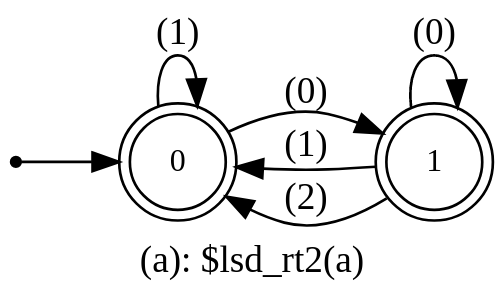
\includegraphics[width=\columnwidth]{lsd_rt2.png}
    \caption{Ostrowski-$\sqrt[~]{2}$ Recognition}
    \label{fig:lsd_rt2}
\end{figure}
\end{minipage}
}

%%%%%%%%%%%%%%%%%%%%%%%%%%%%%%%%%%%%%
%% New Section
%%%%%%%%%%%%%%%%%%%%%%%%%%%%%%%%%%%%%
\section*{The Addition Algorithm and Corresponding Automaton}


An algorithm for addition in Ostrowski numeration systems contains four sub-algorithms. We translated each sub-algorithm into a corresponding automaton which exactly accepts the pairs $(x,y)$ where the algorithm takes in $x$ and gives result $y$.
\begin{itemize}
\item Algorithm 0 simply adds the operands.
\item Algorithm 1 checks constraint 1.
\item Algorithms 2 and 3 check constraint 2.
\end{itemize}
By running the following command in Walnut, we combine our automata for these sub-algorithms, which is shown in \emph{Figure 3}:{
\setlength{\abovedisplayskip}{3pt}
\setlength{\belowdisplayskip}{3pt}
$$\exists y,x,w ~\text{alg}_0(a,b,w) ~\& ~\text{alg}_1(w,x) ~\& ~\text{alg}_2(x,y) ~\& ~\text{alg}_3(y,c)$$}
\begin{mdframed}[style=MyFrame]
\subsection*{Automaton for Algorithm 1}
\end{mdframed}
    \begin{definition}
    $\text{alg}_1(\alpha = [a_0; a_1,a_2,\dots])$ is a nondeterministic finite automaton $\{S,I,T,F\}$ over $\Sigma$ where:
    \begin{itemize}
    \item \textbf{alphabet} $\Sigma = \left\{(s,t) : 0\le s \le 2 ~max(a_i),0\le t \le max(a_i) \right\}$.
   \item set of \textbf{states} $S = \left\{\left(\begin{bmatrix}a&b&c\\d&e&f\end{bmatrix},g,i\right)\right\}$. The matrix represents the input, $g$ is a carry number that is 0 or 1, and $i$ represents the position of $c$ and $f$ in the continued fraction.
   \item set of \textbf{initial states} I = $\left\{\left(\begin{bmatrix}0&0&0\\0&0&0\end{bmatrix},0,i\right)\right\}$ for all integers $i> 0$.
   \item set of \textbf{final states} F = $\left\{\left(\begin{bmatrix}a&b&c\\d&e&f\end{bmatrix},0,0\right):B(a,b,c)=(d,e,f)\right\}$ where $B$ does not change the represented values between $(a,b,c)$ and $(d,e,f)$ while the latter satisfies constraint 1.
   \item \textbf{transition table} :  $\left(\left(\begin{bmatrix}a&b&c\\d&e&f\end{bmatrix},g,i\right), \begin{pmatrix}s\\t\end{pmatrix}, \left(\begin{bmatrix}b'&c'&s'\\e&f&t\end{bmatrix},g',i-1\right)  \right) \in T$ if $(a+g,b,c,s,g)$ and $(d,b',c',s')$ represent the same value, and the latter satisfies constraint 1.
   \end{itemize}
\end{definition}
% \begin{mdframed}[style=MyFrame]
% \subsection*{Automaton for Algorithm 2}
% \end{mdframed}
% \begin{definition}
%     $\text{alg}_2(\alpha = [a_1,a_2,\dots])$ is a nondeterministic finite automaton $\{S,I,T,F\}$ over $\Sigma$ where:
%     \begin{itemize}
%     \item \textbf{alphabet} $\Sigma = \left\{(s,t) : 0\le s,t \le max(a_i) \right\}$
%    \item \textbf{set of states} $S = \left\{\left(\begin{bmatrix}a&b\\c&d\end{bmatrix},i\right)\right\}$. The matrix represents the input,  and $i$ represents the position of $b$ and $d$ in the continued fraction.
%    \item \textbf{initial state} I = $\left\{\left(\begin{bmatrix}0&0\\0&0\end{bmatrix},-2\right)\right\}$.
%    \item \textbf{set of final states} F = $\left\{\left(\begin{bmatrix}a&b\\c&d\end{bmatrix},i\right):a=c,b=d, i\ge0\right\}$.
%    \item \textbf{transition table} :  $\left(\left(\begin{bmatrix}a&b\\c&d\end{bmatrix},i\right), \begin{pmatrix}s\\t\end{pmatrix}, \left(\begin{bmatrix}s'&a'\\t&c\end{bmatrix},i+1\right)  \right) \in T$ if the represented value of $(s,a,b)$ and $(s',a',d)$ are the same, and the latter satisfies constraint 2.
%    \end{itemize}
% \end{definition}

%Here we used \section instead of \section*, so it has a number

\begin{minipage}{.45\columnwidth}
%Insert Picture of automaton

\begin{figure}
	\centering
    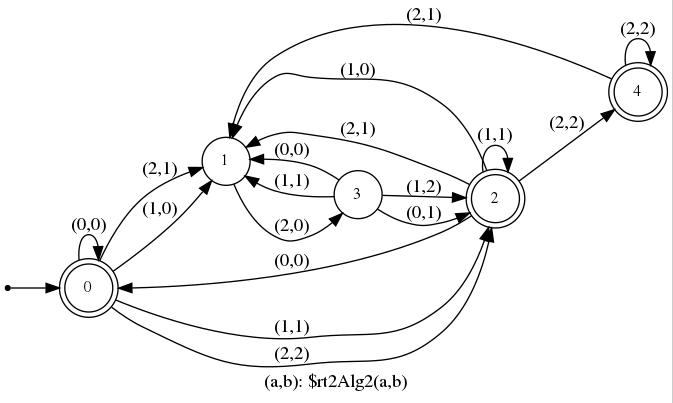
\includegraphics[width=\columnwidth]{rt2Alg2_gv.jpg}
    \caption{Algorithm 2 of Ostrowski-$\sqrt[~]{2}$ (least significant digit first)}
    \label{fig:rt2_alg2}
\end{figure}
\end{minipage} ~~ %
\begin{minipage}{.45\columnwidth}
\begin{figure}
	\centering
    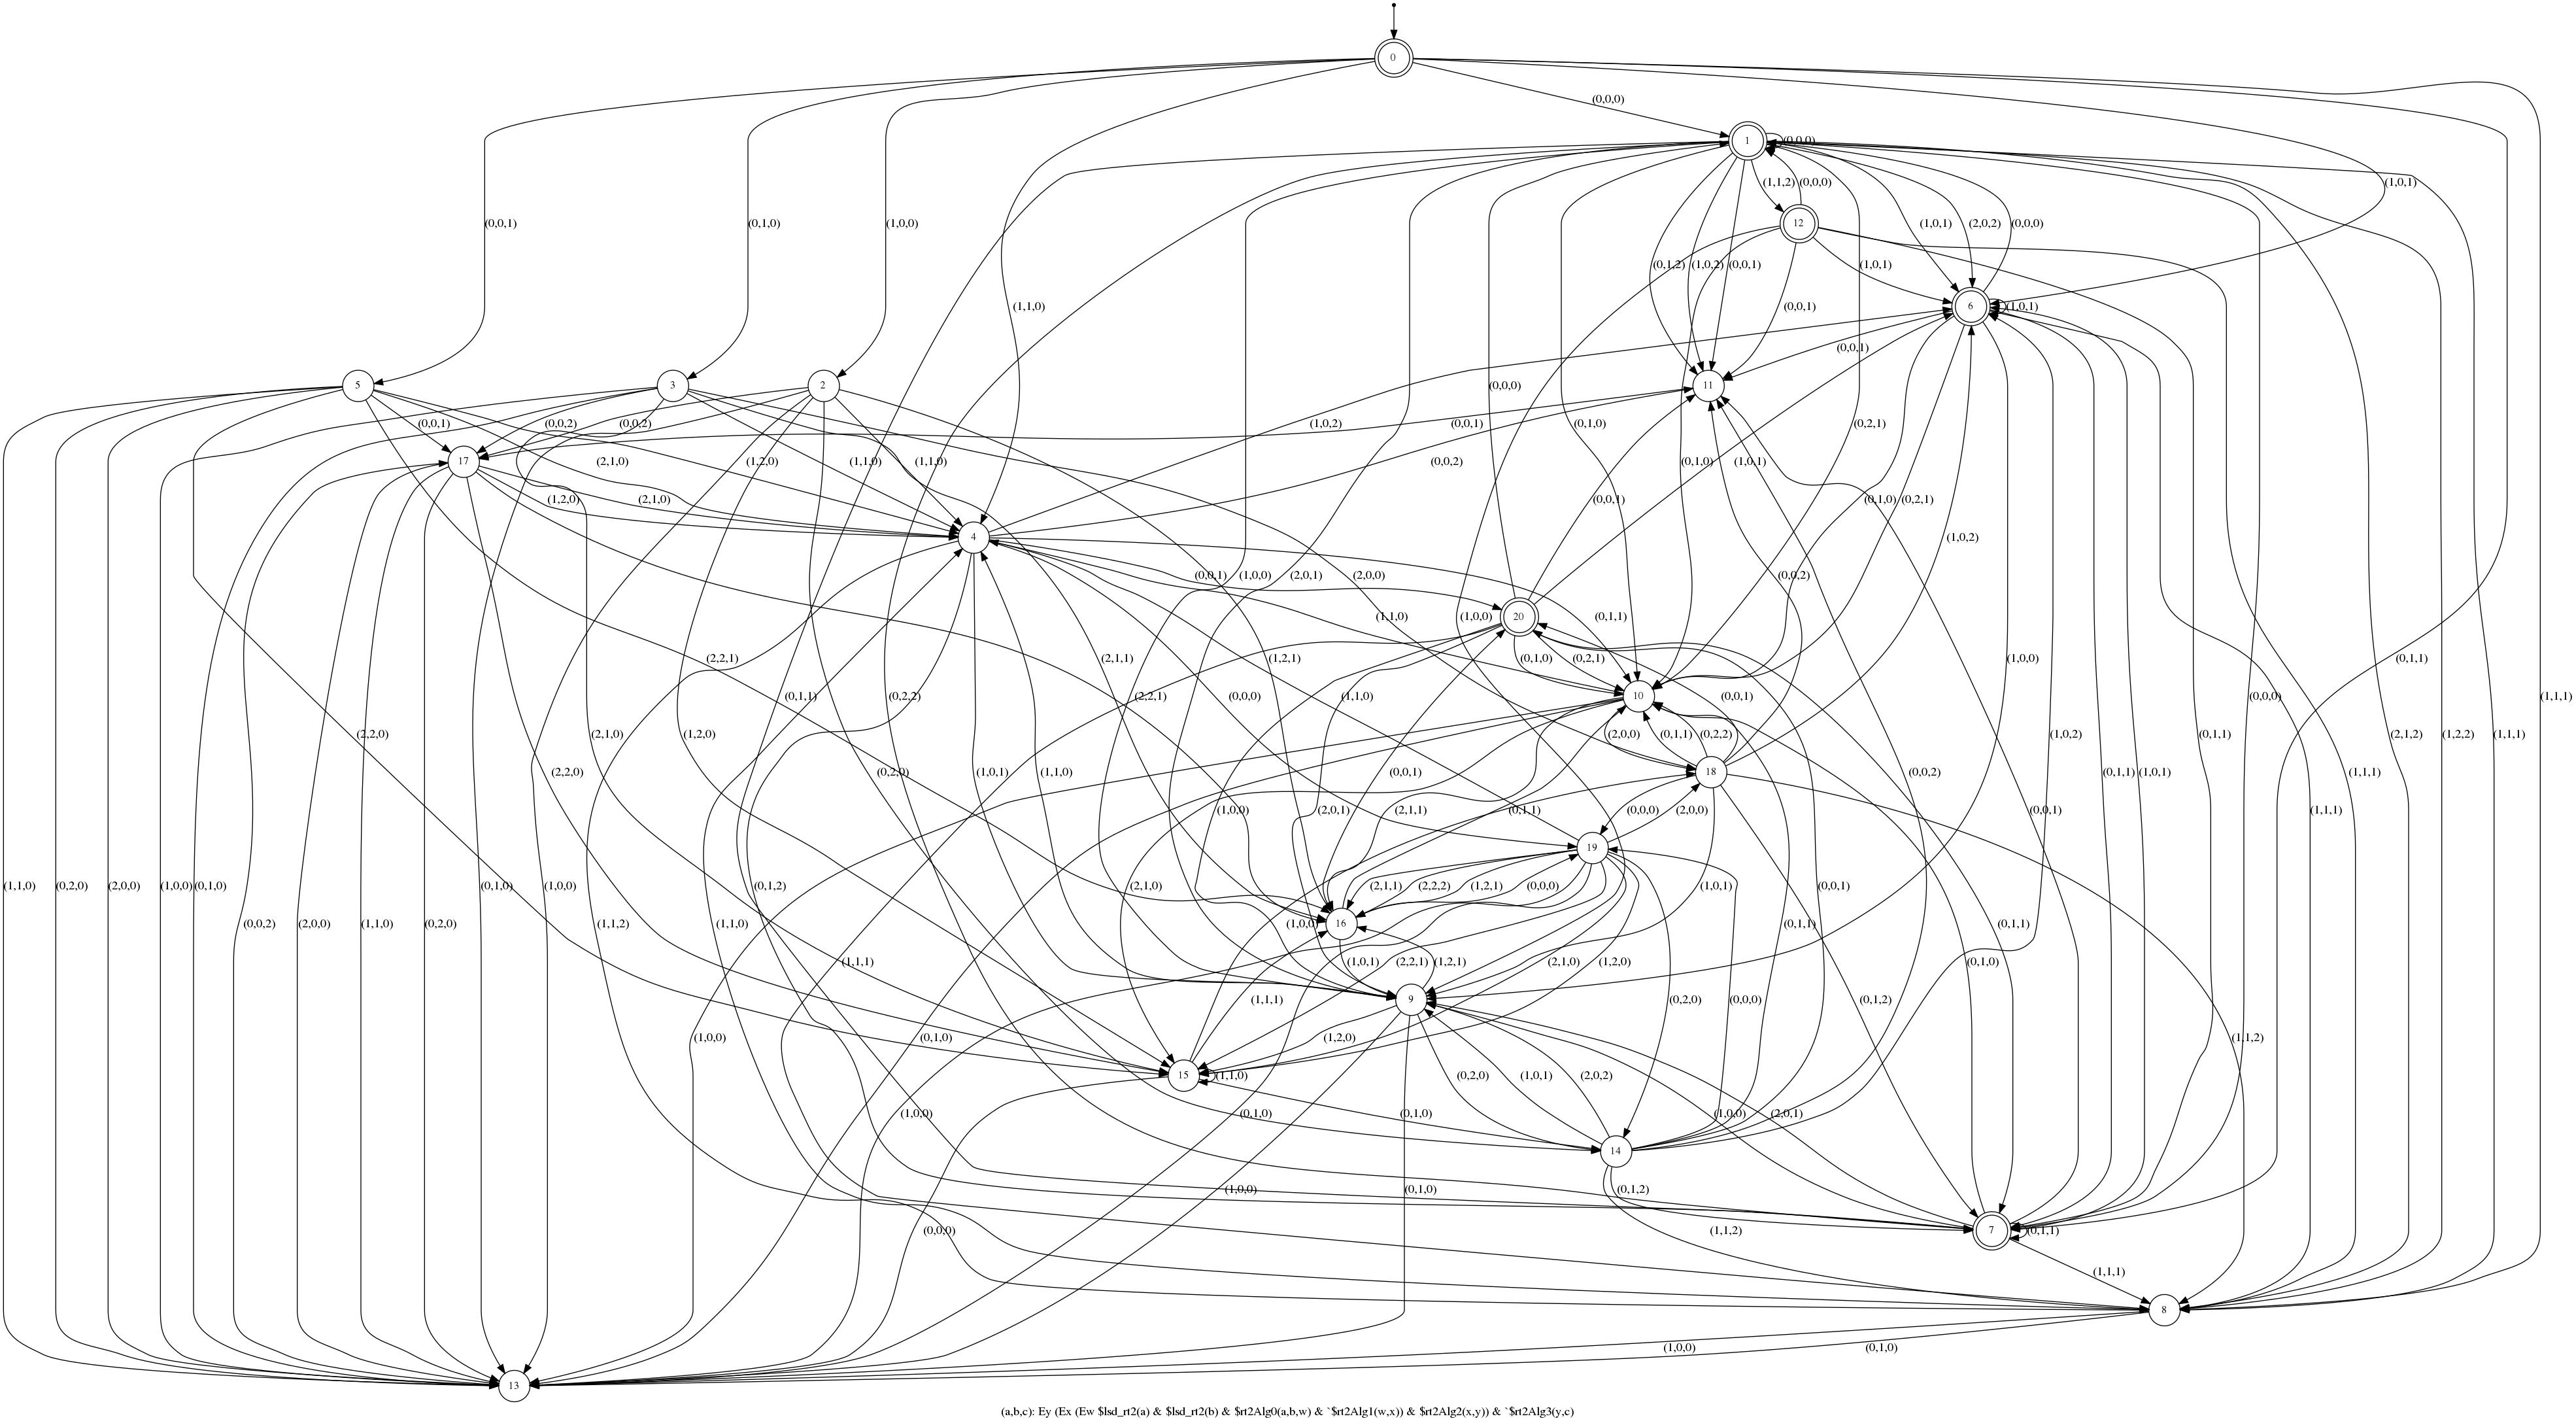
\includegraphics[width=\columnwidth]{lsd_rt2_addition_gv.jpg}
    \caption{Ostrowski-$\sqrt[~]{2}$ Addition}
    \label{fig:rt2_addition}
\end{figure}
\end{minipage}

%%%%%%%%%%%%%%%%%%%%%%%%%%%%%%%%%%%%%
%% New Section
%%%%%%%%%%%%%%%%%%%%%%%%%%%%%%%%%%%%%
\begin{mdframed}[style=MyFrame]
\subsection*{Example of addition algorithm in Ostrowski-$\sqrt[~]{2}$}
\end{mdframed}
\begin{minipage}{\columnwidth}
%Insert explanation of Algorithms 1,2 and 3, etc.

We want to add $103_{10}$ and $132_{10}$ in Ostrowski numeration with $\alpha = \sqrt[~]{2}= [1; 2,2,2,\dots].$
\begin{enumerate}
\item Convert into Ostrowski representation:\\
$109_{10} = 0\times1_{10}+0\times2_{10}+2\times5_{10}+0\times12_{10}+1\times29_{10}+1\times70_{10}= 0110200_{\sqrt[]{2}}$
\\
$138_{10} = 0\times1_{10}+0\times2_{10}+2\times5_{10}+0\times12_{10}+2\times29_{10}+1\times70_{10} = 0120200_{\sqrt[]{2}}$
\item Run Algorithm 0 (add operands): $0110200 + 0120200 \Rightarrow 0230400$.
\item Run Algorithm 1 (check constraint 1): $0230400 \Rightarrow 1020400 \Rightarrow 1021111$.
\item Run Algorithms 2 and 3 (check constraint 2): $1021111 \Rightarrow 1100111$. (Try this on \emph{Figure 2}.)
\end{enumerate}
Therefore, $0110200_{\sqrt[]{2}}+0120200_{\sqrt[]{2}}=1100111_{\sqrt[]{2}}$.\\
Verify:
$1100111_{\sqrt[]{2}}  = 1\times1_{10}+1\times2_{10}+1\times5_{10}+1\times70_{10}+1\times169_{10}$ = $247_{10} = 109_{10}+138_{10}$.\\

\end{minipage}

%%%%%%%%%%%%%%%%%%%%%%%%%%%%%%%%%%%%%
%% New Section
%%%%%%%%%%%%%%%%%%%%%%%%%%%%%%%%%%%%%
\section*{Propositions Evaluated in Walnut}

%include theorems, yay!
With the definition of the automaton for addition in Ostrowski numeration systems, we were able to construct similar proofs as those in Du, Mousavi, Schaeffer, and Shallit's paper "Decision Algorithms for Fibonacci-Automatic Words, with Applications to Pattern Avoidance" for the \textbf{characteristic Sturmian word with slope $\sqrt[~]{2}$} instead of for the original Fibonacci word.
\vspace*{0.4em}
\begin{definition}
The \textbf{characteristic Sturmian word with slope $\sqrt[~]{2}$}, which we denote as $C_2$, is the infinite word obtained as the limit of the sequence of \textbf{standard words} $s_n$ defined by{
\setlength{\abovedisplayskip}{3pt}
\setlength{\belowdisplayskip}{3pt}
$$ s_n=s^{d_n}_{n-1}s_{n-2} \text{ when } n\ge 2, \text{ where } s_1= 0^{d_1-1}1 \text{ and } s_0=0.$$}
\end{definition}
By having built the Ostrowski-$\sqrt[~]{2}$ numeration system and the automatic word $C_2$ in Walnut, we may use the command $C2[i]$ to return the $i^{th}$ digit of $C_2$.\\

\begin{mdframed}[style=MyFrame]
\subsection*{Example theorem}
\end{mdframed}

\textbf{Theorem}: \textbf{$C_2$} \textit{contains fourth powers.}
\\

\textbf{Proof}: We create the following predicate that accepts the length $n$ of fourth powers in $C_2$
\setlength{\abovedisplayskip}{3pt}
\setlength{\belowdisplayskip}{3pt}
$$(n > 0) \land \exists i \; \forall t<3n \;C_2[i+t] = C_2[i+n+t]$$
We then translate the predicate into one that Walnut recognizes:
% \setlength{\abovedisplayskip}{3pt}
% \setlength{\belowdisplayskip}{3pt}
$$ ? \text{msd}\_\text{rt2} ((n>0)~\&~(Ei~At (t<3 \ast n => C2[i+t] = C2[i+n+t])))$$
For this predicate, Walnut generates the following automaton:
\\
\begin{figure}
\centering
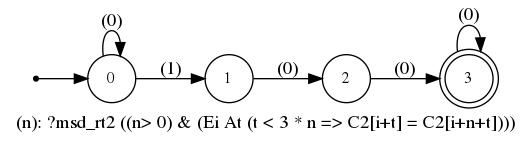
\includegraphics[width=0.7\columnwidth]{theorem5_gv.jpg}
    \caption{Automaton for the Theorem}
    \label{fig:Theorem}
\end{figure}
which means that there are fourth powers of length $100_{\sqrt[~]{2}},1000_{\sqrt[~]{2}},10000_{\sqrt[~]{2}},\dots$.
%Maybe a future work section here?
\section*{Future Work}
\begin{itemize}
\item Use the automata for Ostrowski numeration systems to prove more theorems regarding characteristic Sturmian words.
\item Investigate the critical exponent of infinite balanced words.
\item Find a faster algorithm to generate automata for Ostrowski addition.
\item Provide a general automaton for Ostrowski numeration, which would include $\alpha$ as input.
\end{itemize}

\vspace*{-10pt}  %change to -10
\section*{References}

{\footnotesize [1] Khoussainov, Bakhadyr.Nerode, Anil. (2001) \emph{Automata Theory and its Applications}, MA : Birkh\"auser Boston
}
{\footnotesize [2] Rampersad, Narad. Shallit, Jeffrey and  Vandomme, Elise. (2018) \emph{Critical exponents of infinite balanced words}, Canada
}

{\footnotesize [3] Du, Chen Fei. Mousavi, Hammoon. Schaeffer, Luke and Shallit, Jeffrey. (2014) \emph{Decision Algorithms for Fibonacci-Automatic Words, with Applications to Pattern Avoidance}
}

{\footnotesize [4] Hieronymi, P., \& Terry Jr, A. (2018). \emph{Ostrowski Numeration Systems, Addition, and Finite Automata}. Notre Dame Journal of Formal Logic, 59(2), 215-232.
}

\vspace*{2cm} %This will change to -5
\centerline{\emph{
%Support for this project was provided by the Illinois Geometry Lab and the Department of Mathematics at the University of Illinois at Urbana-Champaign.
}}
\end{multicols}

\end{document}
